\section{Proposed method}\label{sec:yourmethod}

This section defines the scope of our implementation, describes our initial baseline
implementation, analyzes its bottlenecks and outlines the steps which were followed to
increase performance.

\mypar{Scope}
In our project, we focus on grayscale of size $S \times S$, where $S$ is a power of two.
We use quadtree partitioning with maximum depth $7$, error threshold $\epsilon = 300$ and ensure
that the range blocks do not get smaller than $4 \times 4$ pixels which simplifies vectorization.
We furthermore use exhaustive block mapping to search for suitable transformations.

\mypar{Basic implementation}
The baseline is written from scratch in C using an iterative quadtree approach.

Algorithm \ref{alg:baseline} illustrates the compression of the algorithm, whose inputs are the image (row-wise array of doubles) of size $S \times S$,
the max quadtree depth $m$ and the error threshold $\epsilon$.\\
The function \textsc{partition($image$,$s$)} partitions the image into contiguous non-overlapping blocks of size $s \times s$.
The function \textsc{quad($R_i$, $s$)} takes a range block of size $s \times s$ and partitions it into 4 smaller range blocks.
The function \textsc{compute($image$,$R_i$, $D_i$)} computes a transformation with and the resulting RMS according to section \ref{sec:background}. 
Note that the function implicitly rotates the domain block, i.e. the function looks at the four possible locations and returns the transformation with the smallest error.
\begin{algorithm}
\caption{Compression using iterative quadtree}\label{alg:baseline}
\hspace*{\algorithmicindent} \textbf{Input:} $img$ (image of size $S \times S$), $\epsilon$ (RMS threshold) \\
\hspace*{\algorithmicindent} \textbf{Output:} $\boldsymbol{T}$ (set of computed transformations)
\begin{algorithmic}[1]
  \State $\boldsymbol{T} \gets \{\}$ \Comment{Learned transformations} 
  \State $\boldsymbol{R} \gets \Call{partition}{img, S/2}$ \Comment{Initial range blocks} 
    \For{$c=1..m$} \Comment{$c$ is the current quadtree depth}
        \State $\boldsymbol{D} \gets \Call{partition}{img, S/2^{c-1}}$
        \For{$R_i \in \boldsymbol{R}$}
            \State $err_i \gets \infty, T_i \gets \NULL$
            \For{$D_i \in \boldsymbol{D}$}
              \State $T_x, err_x \gets $ \Call{compute}{$img$, $D_i$, $R_i$}
              \If{$err_x < err_i$}
                \State $T_i \gets T_x$
                \State $err_i \gets err_x$
              \EndIf
            \EndFor
        \EndFor
        \State $\boldsymbol{R} \gets \boldsymbol{R} \backslash  R_i$ \Comment{Remove $R_i$ from $\boldsymbol{R}$}
        \If{$err_i > \epsilon$}
          \State $\boldsymbol{R} \gets \boldsymbol{R} \cup  \Call{quad}{R_i, S/2^c}$
        \Else
          \State $\boldsymbol{T} \gets \boldsymbol{T} \cup \{T_i\}$
        \EndIf
    \EndFor
\end{algorithmic}
\end{algorithm}

In order to see if our baseline achieves a reasonable performance, we compared it with
a popular C\texttt{++} implementation from GitHub \cite{github-cpp}. We used the same infrastructure to benchmark
the C\texttt{++} code and our baseline performed slightly better (see !!!ADD LINE TO PERFORMANCEPLOT!!!).

\notejonas{Erwähnen wieso iterativ und nicht rekursiv (memory nicht doppelt so gross)}

\mypar{Scope} For our implementation only square grayscale images with a power
of two width and height were considered. The reason for the restriction on the
size is that it simplifies \textit{Quadtree Partitioning}. If the width of a
range block is a power of two and no suitable transformation is found for it,
then the four new range blocks created by dividing the original range block into
4 equal parts will also have a power of two width. Colored images can be
compressed and decompressed in the same manner as grayscale images.

\notepascal{are we sure about the color stuff?}

\mypar{Roofline} We used the roofline model \cite{applying-roofline} to see whether the algorithm is memory or
compute bound. The peak performance $\pi$ was determined by counting the dispatch
ports specified in the manual \cite{intel-opt-manual}. We distinguish between scalar and vectorized peak
performance. The bandwidth $\beta$ was measured with the STREAM benchmark \cite{stream}. We verified both the peak
performance and the bandwidth with the Empirical Roofline Tool \cite{ert}, which confirmed the values.

For the program model, we need to measure the work $W$, the runtime $T$ and the data move movement $Q$ of
the algorithm. Due to the dynamic nature of quadtree, the model does not only depend on the image size 
but also on the content of the image itself. Therefore, we define the three 
quantities as $W=W(S, img)$, $T=T(S, img)$ and $Q=Q(S, img)$, where $S$ and $img$ are define as in 
\ref{alg:baseline}. We measured $W$ by instrumenting the code according to the cost metric \ref{eq:cost}.
For measuring $T$, we used the \texttt{RDTSC} instruction available on all x86 architecture and disabled
Turbo Boost to guarantee an integer runtime. The measurement of $Q$ is the most challenging and requires
performance counters which are not supported by our hardware. A correct, yet too pessimistic lower bound for $Q$
is $Q \geq 8 \cdot S^2$ because we have to load the image once from memory. One of our group members
developed a tool to simulate a program's memory accesses throughout the course, supporting multi-level caches \cite{github-cache}.\\
We simulated our scalar-optimized code with this tool for the hardware we run our benchmarks on, 
which should give us a tighter lower bound for $Q$. 
This simulation is still too pessimistic for the non-optimized code but more accurate for our scalar-optimized and vectorized code. 
Our experiments showed that for small images ($\leq 512 \times 512$), our theoretical bound holds well. 
It is no surprise that for larger images ($\geq 1024 \times 1024$) the theoretical bound is way too pessimistic
because these images do not entirely fit into L3 cache of our hardware anymore, which leads to more traffic between main memory and cache.

To place the baseline in the roofline plot, we calculated the \textit{operational intensity}
$$
I=\frac{W}{Q}
$$
and the \textit{performance}
$$P=\frac{W}{T}$$
of our implementation. Figure \ref{fig:roofline} shows the 
roofline plot for a specific image with different sizes. One can see that the baseline is inherently compute bound and we have good potential for
performance improvement as the baseline runs only at 12.5\% of scalar peak performance. Next, we use 
profiling to find the performance bottlenecks of the code.

\begin{figure}
  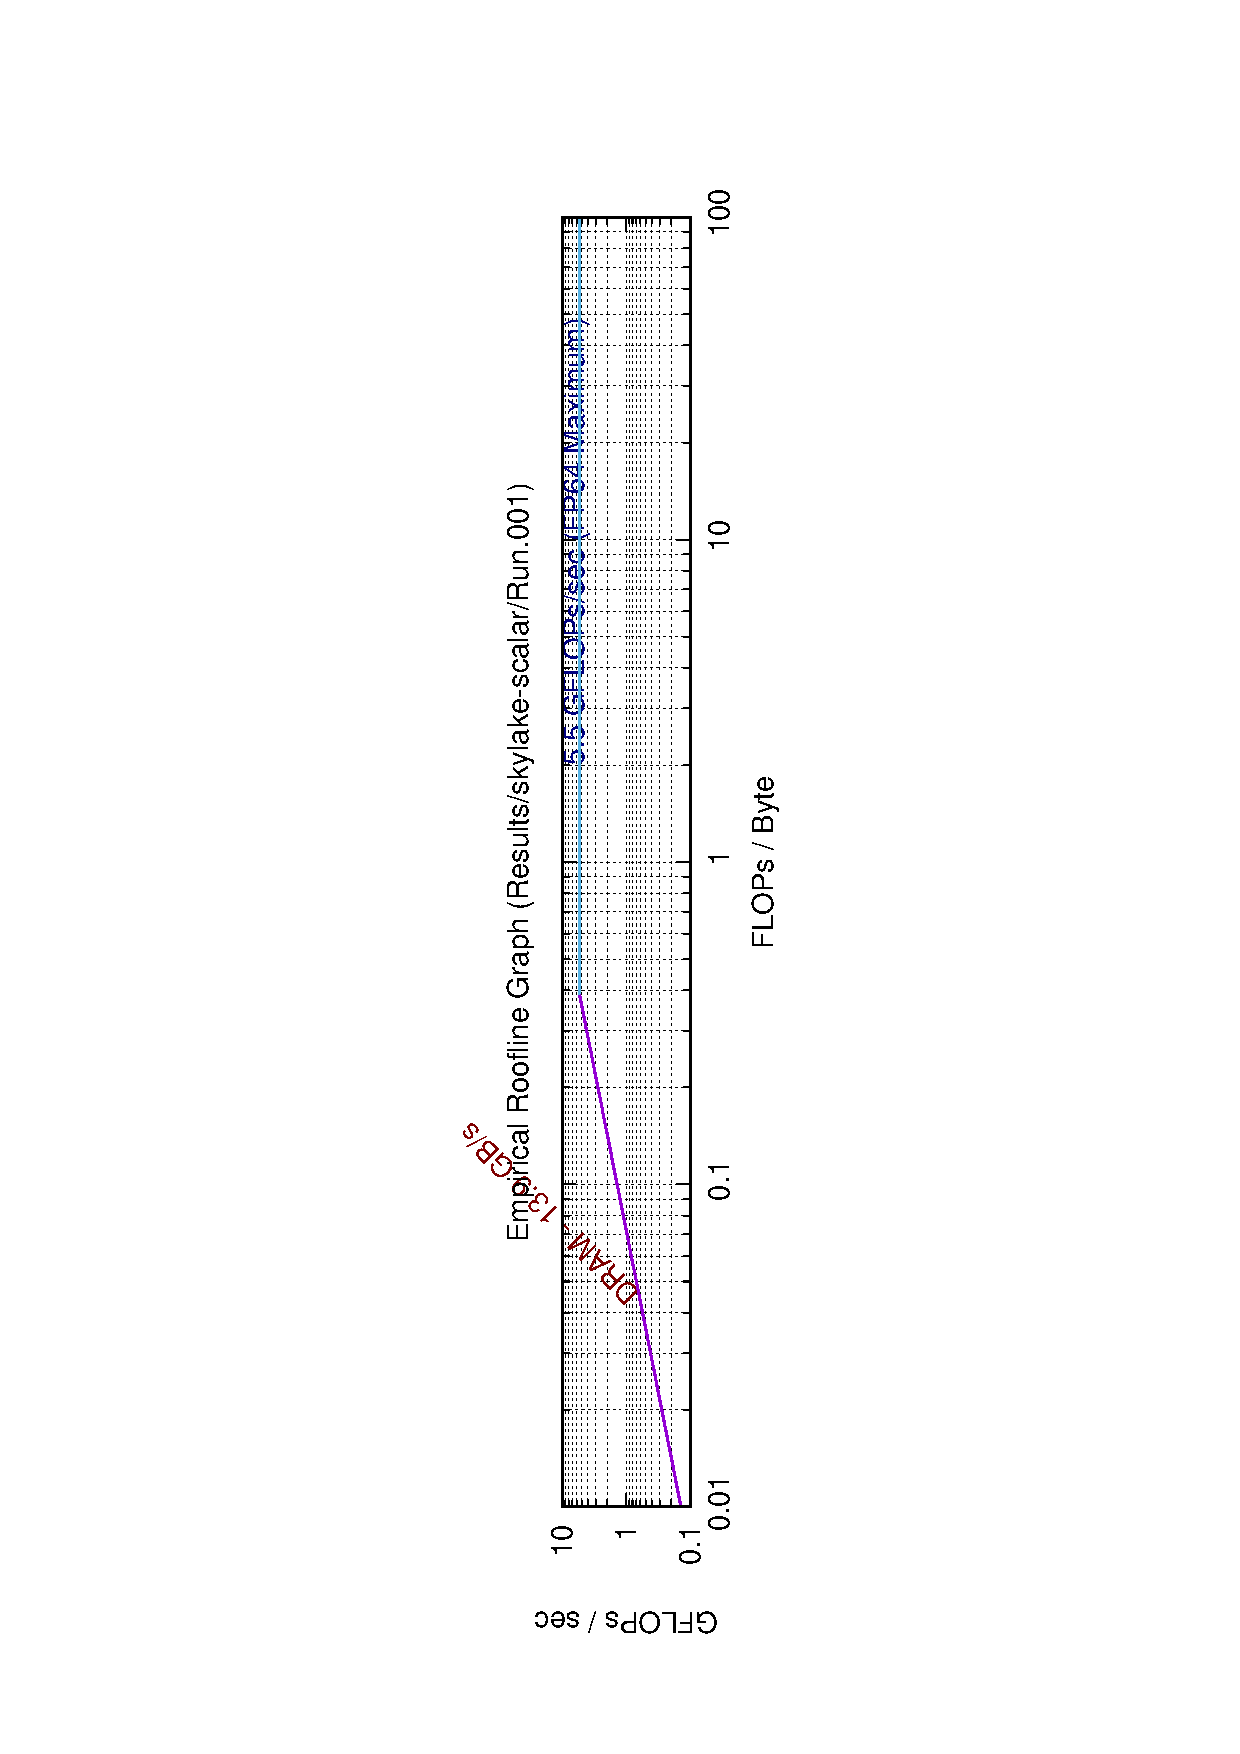
\includegraphics[page=1, width=.45\textwidth]{roofline}
  \caption{Roofline plot for the baseline and various performance optimizations}
  \label{fig:roofline}
\end{figure}

\mypar{Hotspots} A major performance blocker is the exhaustive search for block matches.
In our project, we focus solely on performance, 
whereas using a better search strategy as mentioned in section \ref{sec:intro} is an algorithmic improvement.

When inspecting the code of the baseline, it is apparent that the majority of the work
is done when calculating the contrast, brightness and error of each range/domain block pair 
(equations \ref{contrast}, \ref{brightness} and \ref{error}). We used \textit{Valgrind} 
\cite{valgrind} to profile the code and the profiling report confirmed our assumption. Especially, the sums
over all pixels of a block were identified as hotspots so we started our optimizations there.

\mypar{Scalar Optimizations} As a first optimization we moved the calculation of the sums $\sum_{i=1}^n a_i$, 
$\sum_{i=1}^n a_i^2$, $\sum_{i=1}^n b_i$ and $\sum_{i=1}^n b_i^2$ out of the nested loop 
(see algorithm \ref{alg:baseline} line 5 and 7). The values of these sums change only if the algorithm goes
to the next quadtree depth so we can easily precompute them on each quadtree iteration and reuse them when we
compare each domain block with a range block. This simple precomputation reduced the runtime significantly.

The baseline implementation focused on a clear and understandable code style. Therefore, it uses a queue 
to keep track of the remaining range blocks and several structs to model different concepts of the algorithm 
(e.g. the image). Both the queue and the usage of structs are not optimal for performance so we replaced the
queue and the structs with simple variables and arrays. These changes made the code harder to understand
but eliminated pointer chasing and placed the data better in memory which improves locality.

After the removal of the queue and several structs, we continued with inlining several functions. The inlining
revealed many small optimizations which were not immediately obvious. Another profiling of the optimized
version of the code showed that the computation of $\sum_{i=1}^n a_i b_i$, which is used by the equations 
\ref{contrast} and \ref{error}, is the remaining performance bottleneck. Precomputation of this sum is not possible
because the term depends on values from a specific range and domain block. Thus, we exploit instruction level
parallelism (ILP) to calculate the sum as fast as possible. ILP in combination with scalar replacement and 
optimized array index calculation enabled a faster calculation of this crucial sum which improved overall
performance and runtime significantly.

Finally, we did some experiments with blocking but could not improve performance. We didn't really expect an
improvement as the roofline plot showed that we are compute bound so we abandoned any further experiments in
that direction.

These are all scalar optimizations we applied to the baseline implementation and in the next paragraph we 
discuss further improvements using vector instructions.
\notejonas{Eventuell bei Beginn der Section erwähnen?}
\notejonas{Vielleicht rotationen expliziter erwähnen, dh dass wir die nicht mehr im memory speichern?}

\mypar{Vector Optimizations}

\mypar{Block Rotations}

\mypar{Strided Access}
